\documentclass[12pt,spanish]{article}

\usepackage[left=2.5cm,right=2cm,top=2cm,bottom=2cm]{geometry}
\setlength{\parindent}{0mm}

\usepackage{float}

\usepackage{parskip}
\usepackage[document]{ragged2e}
\usepackage{babel}
\usepackage[utf8]{inputenc}
\usepackage{amsmath,amsthm,mathtools}
\usepackage{amsfonts,amssymb,latexsym}
\usepackage{enumerate}
\usepackage[dvips,usenames]{color}
\definecolor{RojoAnayelRey}{rgb}{1,.25,.25}
\usepackage{tikz}
\usepackage[bookmarks=true,
bookmarksnumbered=false, % true means bookmarks in 
% left window are numbered                         
bookmarksopen=false,     % true means only level 1
% are displayed.
colorlinks=true,
urlcolor=cyan,
linkcolor=blue]{hyperref}

\usepackage{beton}
\usepackage[T1]{fontenc}

\makeatletter
\newcommand{\vast}{\bBigg@{3}}
\newcommand{\Vast}{\bBigg@{4}}
\newcommand{\VAST}{\bBigg@{5.5}}
\makeatother

% Theorem environments

%% \theoremstyle{plain} %% This is the default
\newtheorem{theorem}{Teorema}[section]
\newtheorem{corollary}[theorem]{Corolario}
\newtheorem{lemma}[theorem]{Lema}
\newtheorem{proposition}[theorem]{Proposici\'on}
% \newtheorem{ax}{Axioma}

\theoremstyle{definition}
\newtheorem{definition}{Definici\'on}[section]
\newtheorem{algorithm}{\textrm{\bf Algoritmo}}[section]

% \theoremstyle{remark}
\newtheorem{remark}{Observaci\'on}
\newtheorem{example}{Ejemplo}
\newtheorem{exercise}{Ejercicio}
% \newenvironment{solution}{\begin{proof}[Solution]}{\end{proof}}
\newenvironment{solution}{\begin{proof}[Solución]}{\end{proof}}
\newtheorem*{notation}{Notaci\'on}

\title{Relación 1}

\author{David Cabezas Berrido}

\date{}

\begin{document}
\maketitle

\begin{exercise} Abreviamos $\Sigma=\Sigma_X$ %Ej1
  \begin{enumerate}[a)]
  \item $Y$ sigue una DNM con vector de medias $\alpha$ y matriz de
    covarianzas $D\Sigma D'+\sigma^2 I$, utilizaremos la función
    característica para comprobarlo.
    \[\Phi_Y(t)=E[e^{it'(\alpha+DX+Z)}]=E[e^{it'\alpha}e^{it'DX}e^{it'Z}],\]
    sacamos la constante y utilizamos que $e^{it'DX}$ y $e^{it'Z}$ son
    independientes (funciones medibles de vectores aleatorios
    independientes) para separar las esperanzas,
    \[\Phi_Y(t)=E[e^{it'\alpha}e^{it'DX}e^{it'Z}]=e^{it'\alpha}E[e^{it'DX}]E[e^{it'Z}]=e^{it'\alpha}\Phi_X(D't)\Phi_Z(t).\]
    Sustituimos las funciones características de $X$ y $Z$ para
    obtener lo que queríamos:
    \[\Phi_Y(t)=e^{it'\alpha}\exp\left\{-\frac{1}{2}t'D\Sigma
        D't\right\}\exp\left\{-\frac{1}{2}t'\sigma^2 I
        t\right\}=\exp\left\{it'\alpha -\frac{1}{2}t'\big(D\Sigma
        D'+\sigma^2I\big)t\right\}.\] Por tanto,
    $Y\sim N_p\big(\alpha,D\Sigma D'+\sigma^2I\big)$.
  \item Utilizando que $X$ y $Z$ son independientes y siguen ambas una
    $DNM$ no singular, obtenemos para cada $\begin{psmallmatrix}
      t_1 \\ t_2
    \end{psmallmatrix}\in\mathbb{R}^{p+r}$ 
    \begin{align*}
      \Phi_{
      \begin{psmallmatrix}
        Z \\ X
      \end{psmallmatrix}
      }
      \begin{psmallmatrix}
        t_1 \\ t_2
      \end{psmallmatrix}
      &=\Phi_Z(t_1)\Phi_X(t_2)=\exp\left\{-\frac{1}{2}t_1'\sigma^2 It_1\right\}\exp\left\{-\frac{1}{2}t_2'\Sigma t_2\right\} \\
      &=\exp\left\{-\frac{1}{2}\big(\sigma^2 t_1't_1+t_2'\Sigma t_2\big)\right\}=\exp\left\{-\frac{1}{2}
        \begin{pmatrix}
          t_1' & t_2'
        \end{pmatrix}
                 \begin{pmatrix}
                   \sigma^2I & 0 \\ 0 & \Sigma
                 \end{pmatrix}
                                        \begin{pmatrix}
                                          t_1 \\ t_2
                                        \end{pmatrix}
      \right\}
    \end{align*}
    Por tanto, $\begin{pmatrix} Z \\ X
    \end{pmatrix}\sim N_{p+r}\left(0,
      \begin{pmatrix}
        \sigma^2I & 0 \\ 0 & \Sigma
      \end{pmatrix}
    \right)$.

    Utilizando, el Resultado para transformaciones lineales de rango
    máximo para DNM caso no singular, obtenemos que
    \[
      \begin{pmatrix}
        Y \\ X
      \end{pmatrix}=
      \begin{pmatrix}
        \alpha+DX+Z \\ X
      \end{pmatrix}=
      \begin{pmatrix}
        I & D \\ 0 & I
      \end{pmatrix}
      \begin{pmatrix}
        Z \\ X
      \end{pmatrix}+
      \begin{pmatrix}
        \alpha \\ 0
      \end{pmatrix}
    \]
    sigue una distribución normal multivariante con vector de medias $
    \begin{pmatrix}
      \alpha \\ 0
    \end{pmatrix}$ y matriz de covarianzas $
    \begin{pmatrix}
      I & D \\ 0 & I
    \end{pmatrix}\begin{pmatrix}
      \sigma^2I & 0 \\ 0 & \Sigma
    \end{pmatrix}\begin{pmatrix}
      I & 0 \\ D' & I
    \end{pmatrix}=
    \begin{pmatrix}
      D\Sigma D'+\sigma^2I & D\Sigma \\ \Sigma D' & \Sigma
    \end{pmatrix}$.
  \item $\begin{pmatrix}
      Y \\ X
    \end{pmatrix}$ sigue una DNM con matriz de covarianzas definida
    positiva, usamos por tanto el Resultado 3 de DNM no
    singular. Obtenemos que la distribución condicionada de $X$ a
    $Y=y$ sigue una DNM de la forma:
    \[N_r\Big(0+\Sigma D'(D\Sigma
      D'+\sigma^2I)^{-1}(y-\alpha),\Sigma-\Sigma D'(D\Sigma
      D'+\sigma^2I)^{-1}D\Sigma\Big)\] Así, que
    $E[X|Y]=\Sigma D'(D\Sigma D'+\sigma^2I)^{-1}(Y-\alpha)=\Sigma D'\Sigma_Y^{-1}(Y-\alpha)$
  \item Utilizamos el mismo resultado, pero cambiamos los papeles de
    $X$ e $Y$, obteniendo que $Y$ condicionado a $X$ sigue una DNM
    con vector de medias
    \[\alpha+D\Sigma\Sigma^{-1}(X-0)\]
    y matriz de covarianzas
    \[D\Sigma D'+\sigma^2I-D\Sigma\Sigma^{-1}\Sigma D'\]
    Simplificando, obtenemos
    \[Y|X\sim N_p\Big(\alpha+D X,\sigma^2I\Big)\]
  \end{enumerate}
\end{exercise}

\begin{exercise} \label{ej2} %Ej2
  Especificaremos los matices que cambian en los argumentos
  anteriores.
  \begin{enumerate}[a)] 
  \item El razonamiento es también válido para $\Sigma\geq 0$.
  \item Aunque transformación lineal que utilizamos sigue siendo de
    rango máximo, el Resultado sobre transformaciones lineales de
    rango no necesariamente máximo proporciona las mismas conclusiones
    también en el caso de que $
    \begin{pmatrix}
      Z \\ X
    \end{pmatrix}$ siga una DNM con matriz de covarianzas semidefinida
    positiva, lo que ocurre cuando $\Sigma$ sólo es semidefinida
    positiva.
  \item Ahora (caso singular) el resultado sobre condicionamiento nos
    da:
    \[X|Y\sim N_r\Big(0+\Sigma D'(D\Sigma
      D'+\sigma^2I)^-(y-\alpha),\Sigma-\Sigma D'(D\Sigma
      D'+\sigma^2I)^-D\Sigma\Big)\] Ahora probaremos que
    $\Sigma_Y=D\Sigma D'+\sigma^2I$ es definida positiva y por tanto
    regular: si $y\in \mathbb{R}^p\backslash\{0\}$,
    $y'\Sigma_Y y=y'(D\Sigma D'+\sigma^2I)y=y'D\Sigma
    D'y+y'\sigma^2Iy=y'D\Sigma D'y+\sigma^2\|y\|_2^2>y'D\Sigma D'y\geq
    0$, ya que $D\Sigma D'$ es semidefinida positiva. Por tanto,
    $\Sigma_Y$ tiene inversa y $\Sigma_Y^-=\Sigma_Y^{-1}$. Lo que nos
    permite concluir el ejercicio tenemos lo que queremos.
  \item Ahora el resultado sobre condicionamiento nos proporciona
    \[Y|X\sim N_p\Big(\alpha+D\Sigma\Sigma^-X,D\Sigma
      D'+\sigma^2I-D\Sigma\Sigma^-\Sigma D'\Big)\] Simplificando
    $\Sigma\Sigma^-\Sigma=\Sigma$, y cancelando $D\Sigma D'$ obtenemos
    \[Y|X\sim N_p\Big(\alpha+D\Sigma\Sigma^-X,\sigma^2I\Big)\]
  \end{enumerate}
\end{exercise}

\begin{exercise} %Ej3

  Debemos tener en cuenta que $\alpha'(X-\mu)$ es una variable
  aleatoria unidimensional.
  
  Si $k=0$, el resultado es obvio: $E[1]=1$, ya que $m=\frac{k}{2}=0$
  y $0!=a^0=1$ para cualquier número real $a$. Suponemos en adelante
  $k>0$.
  
  Si $\alpha=0$, obtenemos otra trivialidad: $E[0]=0$. De lo
  contrario, podemos ver $\alpha'$ como una matriz $1\times p$ de
  rango máximo y aplicar el resultado sobre transformaciones lineales
  de rango máximo (Resultado 4 de DNM para $\Sigma>0$) para concluir
  $Y\sim
  N(\alpha'\mu-\alpha'\mu,\alpha'\Sigma\alpha'')=N(0,\alpha'\Sigma\alpha)$.
  
  El resultado auxiliar nos proporciona entonces $E[Y^k]=0$ para $k$
  impar y \\ $E[Y^k]=(\alpha'\Sigma\alpha)^\frac{k}{2} (k-1)!!$,
  sustituyendo $m=\frac{k}{2}$ obtenemos
  $E[Y^k]=(\alpha'\Sigma\alpha)^m (2m-1)!!$ y sólo queda probar
  $(2m-1)!!=\frac{(2m)!}{2^m m!}$ para todo $m\in\mathbb{N}$,
  $m\geq 1$. Esto lo haremos por inducción sobre $m$:
  
  En el caso $m=1$ basta desarrollar y obtenemos
  \[(2\cdot 1-1)!!=1!!=1;\qquad \frac{(2\cdot 1)!}{2^1
      1!}=\frac{2}{2}=1\] Supuesta la igualdad para $m-1$, es decir,
  \[(2m-3)!!=\big(2(m-1)-1\big)!!=\frac{\big(2(m-1)\big)!}{2^{m-1} (m-1)!}=\frac{(2m-2)!}{2^{m-1} (m-1)!}.\]

  Comprobamos para $m$,
  \begin{align*}
    &(2m-1)!!=\frac{(2m)!}{2^m m!}
      \Longleftrightarrow (2m-1)(2m-3)!!=\frac{(2m)!}{2^m m!} \\
    \xLeftrightarrow[m-1]{\text{Caso}}\quad &(2m-1)\frac{(2m-2)!}{2^{m-1}(m-1)!}=\frac{(2m)!}{2^m m!} \Longleftrightarrow (2m-1)!=\frac{(2m)!}{2m}
  \end{align*}
  y obtenemos lo que queríamos.
  
\end{exercise}

\begin{exercise} %Ej4
  De que $H$ sea ortogonal, obtenemos
  \[I_p=HH'=
    \begin{pmatrix}
      H_1 & H_2
    \end{pmatrix}
    \begin{pmatrix}
      H_1' \\ H_2'
    \end{pmatrix}=H_1H_1'+H_2H_2'
  \]
  \[I_p=H'H=
    \begin{pmatrix}
      H_1' \\ H_2'
    \end{pmatrix}
    \begin{pmatrix}
      H_1 & H_2
    \end{pmatrix}=
    \begin{pmatrix}
      H_1'H_1 & H_1'H_2 \\ H_2'H_1 & H_2'H_2
    \end{pmatrix}
  \]
  También sabemos que $\Sigma=H_1DH_1'$.
  \begin{enumerate}[a)]
  \item \[\Sigma\Sigma^+\Sigma=H_1DH_1'H_1D^{-1}H_1'H_1DH_1'\]
    Usando que $H_1'H_1=I_k$,
    \[\Sigma\Sigma^+\Sigma=H_1DD^{-1}DH_1'=H_1DH_1'=\Sigma\]
  \item \[\Sigma^+\Sigma\Sigma^+=H_1D^{-1}H_1'H_1DH_1'H_1D^{-1}H_1'\]
    De nuevo usando $H_1'H_1=I_k$,
    \[\Sigma^+\Sigma\Sigma^+=H_1D^{-1}DD^{-1}H_1'=H_1D^{-1}H_1'=\Sigma^+\]
  \item Utilizamos que tanto $\Sigma$ como $\Sigma^+$ son
    simétricas, y otra vez más que $H_1'H_1=I_k$:
    \[(\Sigma^+\Sigma)'=\Sigma\Sigma^+=H_1DH_1'H_1D^{-1}H_1'=H_1H_1'\]
    Por otra parte
    \[\Sigma^+\Sigma=H_1D^{-1}H_1'H_1DH_1'=H_1D^{-1}DH_1'=H_1H_1'\]
  \item $(\Sigma\Sigma^+)=\Sigma^+\Sigma$, que por el apartado
    anterior sabemos que coincide con $\Sigma\Sigma^+$.
  \end{enumerate}
\end{exercise}

\begin{exercise} %Ej5
  \[\Sigma=
    \begin{pmatrix}
      1 & 0 & \sigma_{13} \\
      0 & 1 & \sigma_{23} \\
      \sigma_{13} & \sigma_{23} & 1
    \end{pmatrix}
  \]

  Los menores de orden 1 y 2 de la diagonal principal de $\Sigma$
  valen los dos $1>0$, luego $\Sigma$ es definida positiva si, y solo
  si su determinante es positivo. Hemos de probar por tanto
  $0\geq|\Sigma|=1-\sigma_{13}^2-\sigma_{23}^2$, sabiendo que
  $\sigma_{13}+\sigma_{23}>\frac{3}{2}$. Por comodidad, renombramos
  $\sigma_{13}=x$, $\sigma_{23}=y$; queremos probar $x^2+y^2\geq 1$
  para $x+y>\frac{3}{2}$.

  Geométricamente, esto no es más que decir que el semiplano abierto
  $P:x+y>\frac{3}{2}$ está contenido en el complementario del disco
  abierto unidad $D:x^2+y^2 < 1$, o lo que es lo mismo,
  $P\cap D=\emptyset$. En esta figura se ve claramente
  \begin{figure}[H]
    \centering
    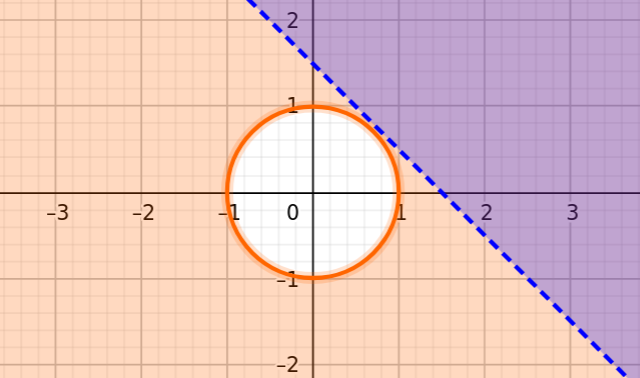
\includegraphics[width=80mm]{ej1-5.png}
  \end{figure}

  Haremos una demostración analítica, la función
  $f(x,y)=x^2+y^2\geq 0$ está minorada y por tanto tiene ínfimo no
  negativo en el conjunto $P$. Caben tres posibilidades:
  \begin{itemize}
  \item El ínfimo se alcanza en un punto interior donde se anula el
    gradiente, pero $\nabla f(x,y)=2(x,y)\neq(0,0)$ en $P$.
  \item El ínfimo se alcanza en la frontera de $P$, donde
    $y=\frac{3}{2}-x$. $f(x,\frac{3}{2}-x)=2x^2-3x+\frac{9}{4}$, que
    es mínimo en $x=\frac{3}{4}$ y vale $1.125>1$.
  \item Existe una sucesión divergente cuya imagen por $f$ converge al
    ínfimo, esto no puede darse puesto que $f$ es el cuadrado de la
    norma euclídea.
  \end{itemize}

  De esto deducimos que $\inf\{f(x,y) : (x,y)\in P\}=1.125$ y puesto
  que $P$ no contiene a su frontera, $x^2+y^2>1.125$ en todo $P$. Y
  por tanto $|\Sigma|\leq 0$, por lo que $\Sigma$ no puede ser
  definida positiva.
\end{exercise}

\begin{exercise} % Ej6
  Dado $Z\sim_p(0,I_p)$, debemos encontrar una condición necesaria y
  suficiente para las dos matrices $k_i\times p$, $C_i$, con
  $k_i\leq p$ para $i=1,2$, que caracterice la independencia de
  $Y_1=C_1 Z$ e $Y_2=C_2 Z$.

  Partimos de la caracterización de independencia por medio de la
  función característica: $Y_1$ e $Y_2$ son independientes si y solo si
  \begin{equation} \label{indep-caracteristica}
    \Phi_{
      \begin{psmallmatrix}
        Y_1 \\ Y_2
      \end{psmallmatrix}
    }(t)=\Phi_{Y_1}(t_1)\Phi_{Y_2}(t_2),\quad\text{para todo } t=\begin{pmatrix}
      t_1 \\ t_2
    \end{pmatrix}\in\mathbb{R}^{k_1+k_2}
  \end{equation}
  Utilizamos el resultado para transformaciones lineales de rango no
  necesariamente máximo para el caso $\Sigma\geq 0$, y obtenemos que
  \[\begin{pmatrix}
      C_1 \\ C_2
    \end{pmatrix}Z=\begin{pmatrix}
      C_1 Z \\ C_2 Z
    \end{pmatrix}=\begin{pmatrix}
      Y_1 \\ Y_2
    \end{pmatrix}\]
  cumple
  \[\begin{pmatrix}
      Y_1 \\ Y_2
    \end{pmatrix}\sim N_{k_1+k_2}\vast(0,\begin{pmatrix}
      C_1 \\ C_2
    \end{pmatrix} I_p \begin{pmatrix}
      C_1' & C_2'
    \end{pmatrix}\vast)\]
  Llamando \[C=\begin{pmatrix}
      C_1 \\ C_2
    \end{pmatrix} I_p \begin{pmatrix}
      C_1' & C_2'
    \end{pmatrix}=\begin{pmatrix}
      C_1 C_1' & C_1 C_2' \\ C_2 C_1' & C_2 C_2'
    \end{pmatrix}\]
  tenemos que \[\Phi_{
      \begin{psmallmatrix}
        Y_1 \\ Y_2
      \end{psmallmatrix}
    }(t)=\exp\left\{-\frac{1}{2}t'Ct\right\}\]
  De forma análoga, tenemos para $Y_i=C_i Z$ ($i=1,2$)
  \[Y_i\sim N_{k_i}(0,C_i I C_i'),\] por tanto
  \[\Phi_{Y_i}(t_i)=\exp\left\{-\frac{1}{2}t_i'C_iC_i't_i\right\}\]
  (\ref{indep-caracteristica}) queda ahora así:
  \[\exp\left\{-\frac{1}{2}t'Ct\right\}=\exp\left\{-\frac{1}{2}t_1'C_1C_1't_1\right\}\exp\left\{-\frac{1}{2}t_2'C_2C_2't_2\right\},\quad\text{para todo } t=\begin{pmatrix}
      t_1 \\ t_2
    \end{pmatrix}\in\mathbb{R}^{k_1+k_2}\]
  Y la inyectividad de la exponencial nos dice que la independencia
  entre $Y_1$ e $Y_2$ equivale a
  \[t'Ct=t_1'C_1C_1't_1+t_1'C_1C_1't_1\quad\text{para todo }
    t=\begin{pmatrix} t_1 \\ t_2
    \end{pmatrix}\in\mathbb{R}^{k_1+k_2}\]
  Desarrollando, obtenemos
  \[t'Ct=
    \begin{pmatrix}
      t_1' & t_2'
    \end{pmatrix}
    \begin{pmatrix}
      C_1 C_1' & C_1 C_2' \\ C_2 C_1' & C_2 C_2'
    \end{pmatrix}
    \begin{pmatrix}
      t_1 \\ t_2
    \end{pmatrix}=t_1'C_1C_1't_1+t_1'C_1C_2't_2+t_2'C_2C_1't_1+t_2'C_2C_2't_2\]
  Por tanto, $Y_1$ e $Y_2$ son independientes si y solo si
  \[t_1'C_1C_2't_2+t_2'C_2C_1't_1=0,\quad\text{para todo }
    \begin{pmatrix} t_1 \\ t_2
    \end{pmatrix}\in\mathbb{R}^{k_1+k_2}\]
  Tenemos la suma de dos escalares, así que podemos trasponer uno:
  $t_2'C_2C_1't_1=(t_2'C_2C_1't_1)'=t_1'C_1C_2't_2$. Obteniendo así \begin{equation} \label{indep-condition} t_1'C_1C_2't_2=0,\quad\text{para todo }
    \begin{pmatrix} t_1 \\ t_2
    \end{pmatrix}\in\mathbb{R}^{k_1+k_2}\end{equation}
  Claramente esto se satisface cuando $C_1C_2'=0$. Recíprocamente, si
  $C_1C_2'=(d_{ij})$ tuviese una entrada $d_{ij}\neq 0$ para algunos
  $i=1,\ldots,k_1$, $j=1,\ldots,k_2$, tomando $t_1(n)=
  \begin{cases}
    1 \text{ si } n=i \\
    0 \text{ en otro caso}
  \end{cases}
  $ y $t_2(n)=
  \begin{cases}
    1 \text{ si } n=j \\
    0 \text{ en otro caso}
  \end{cases}
  $ tendríamos $t_1'C_1C_2't_2=d_{ij}\neq 0$, luego
  (\ref{indep-condition}) equivale a que $C_1C_2'=0$. Por tanto, $Y_1$
  e $Y_2$ son independientes si y solo si $C_1C_2'=0$.
\end{exercise}

\begin{exercise} % Ej7 
  $Y\sim N_3(\mu,\Sigma)$, con
  \[\mu=
    \begin{pmatrix}
      3 \\
      1 \\
      4
    \end{pmatrix},\qquad \Sigma=
    \begin{pmatrix}
      6 & 1 & -2 \\
      1 & 13 & 4 \\
      -2 & 4 & 4
    \end{pmatrix}
  \]

  $|\Sigma|=144>0$ y $\Sigma$ simétrica. Luego es definida
  positiva. La idea de los apartados a-e es escribir la variable que
  queremos estudiar como una transformada lineal de rango máximo de
  $Y$ y aplicar el resultado de transformaciones lineales de rango
  máximo para $\Sigma>0$.
  
  \begin{enumerate}[a)]
  \item \[Z=2Y_1-Y_2+3Y_3=
      \begin{pmatrix}
        2 & -1 & 3
      \end{pmatrix}
      Y
    \]
    Como la matriz $B=\begin{pmatrix}
      2 & -1 & 3
    \end{pmatrix}$ tiene rango 1, el resultado sobre
    transformaciones lineales de máximo rango para $\Sigma>0$ nos
    asegura que $Z\sim N_1(B\mu,B\Sigma B')=N_1(17,21)$.
  \item $(Z_1,Z_2)$ donde $Z_1=Y_1+Y_2+Y_3$, $Z_2=Y_1-Y_2+2Y_3$.
    \[\begin{pmatrix}
        Z_1 \\
        Z_2
      \end{pmatrix}
      =\begin{pmatrix}
        1 & 1 & 1 \\
        1 & -1 & 2
      \end{pmatrix}Y=BY
    \]
    Esta vez el rango de $B=\begin{pmatrix}
      1 & 1 & 1 \\
      1 & -1 & 2
    \end{pmatrix}$ es 2, y el mismo resultado nos da \\ $\begin{pmatrix}
      Z_1 \\
      Z_2
    \end{pmatrix}\sim N_2\left(
      \begin{pmatrix}
        8 \\ 10
      \end{pmatrix},
      \begin{pmatrix}
        29 & -1 \\
        -1 & 9
      \end{pmatrix}\right)$.
  \item \[Y_2=
      \begin{pmatrix}
        0 & 1 & 0
      \end{pmatrix}
      Y=BY
    \]
    El rango de $B$ sigue siendo máximo, por tanto $Y_2\sim N_1(1,13)$.
  \item \[\begin{pmatrix}
        Y_1 \\
        Y_3
      \end{pmatrix}
      =\begin{pmatrix}
        1 & 0 & 0 \\
        0 & 0 & 1
      \end{pmatrix}Y\] Una vez más el mismo resultado nos dice
    que $\begin{pmatrix}
      Y_1 \\
      Y_2
    \end{pmatrix}\sim N_2\left(
      \begin{pmatrix}
        3 \\ 4
      \end{pmatrix},
      \begin{pmatrix}
        6 & -2 \\
        -2 & 4
      \end{pmatrix}\right)$.
  \item \[\begin{pmatrix}
        Y_1 \\
        Y_3 \\
        \frac{1}{2}(Y_1+Y_2)
      \end{pmatrix}
      =\begin{pmatrix}
        1 & 0 & 0 \\
        0 & 0 & 1 \\
        \frac{1}{2} & \frac{1}{2} & 0
      \end{pmatrix}Y\]
    $\begin{pmatrix}
      Y_1 \\
      Y_3 \\
      \frac{1}{2}(Y_1+Y_2)
    \end{pmatrix}\sim N_3\left(
      \begin{pmatrix}
        3 \\ 4 \\ 2
      \end{pmatrix},
      \begin{pmatrix}
        6 & -2 & \frac{7}{2} \\
        -2 & 4 & 1 \\
        \frac{7}{2} & 1 & \frac{21}{4}
      \end{pmatrix}\right)$.
  \item Encontrar $Z$ tal que $Z=(T')^{-1}(Y-\mu)\sim N_3(0,I)$. Con
    $T$ la matriz correspondiente a la factorización de Cholesky,
    $\Sigma=T'T$.

    Utilizamos el algoritmo para la descomposición de Cholesky
    implementado en la herramienta \href{https://www.sagemath.org}{\texttt{SageMath}}, y obtenemos
    que (redondeando)
    \[\Sigma=T'T=
      \begin{pmatrix}
        2.4495 & 0 & 0 \\
        0.4082 & 3.5824 & 0 \\
        -0.8165 & 1.2096 & 1.3675
      \end{pmatrix}
      \begin{pmatrix}
        2.4495 & 0.4082 & -0.8165 \\
        0 & 3.5824 & 1.2096 \\
        0 & 0 & 1.3675
      \end{pmatrix}
    \]
    También con \texttt{SageMath}, calculamos la inversa:
    \[T^{-1}=\begin{pmatrix}
        0.4082 & -0.0465 & 0.2849 \\
        0 & 0.2791 & -0.2469 \\
        0 & 0 & 0.7312
      \end{pmatrix}\]
    Luego \[Z=\begin{pmatrix}
        0.4082 & -0.0465 & 0.2849 \\
        0 & 0.2791 & -0.2469 \\
        0 & 0 & 0.7312
      \end{pmatrix}\left(Y-\mu\right)\]
    Como $T'T=\Sigma$, se tiene $Z\sim N_3(0,I)$.
  \item Encontrar $Z$ tal que
    $Z=\Sigma^{-\frac{1}{2}}(Y-\mu)\sim N_3(0,I)$. Con
    $\Sigma^{-\frac{1}{2}}$ la inversa de la matriz correspondiente
    a la factorización raíz cuadrada,
    $\Sigma=\Sigma^\frac{1}{2}\Sigma^\frac{1}{2}$.

    Con la función
    \href{https://numpy.org/doc/stable/reference/generated/numpy.linalg.eigh.html}{\texttt{np.linalg.eigh}},
    obtenemos una matriz ortogonal
    \[V=
      \begin{pmatrix}
        -0.4358 & 0.8996 & 0.0276 \\
        0.3268 & 0.1296 & 0.9362 \\
        -0.8386 & -0.417 & 0.3505
      \end{pmatrix}
    \] que cumple \[V'\Sigma V=
      \begin{pmatrix}
        1.4018 & 0 & 0 \\
        0 & 7.0712 & 0 \\
        0 & 0 & 14.527
      \end{pmatrix}=D\]
    Tomando \[D^\frac{1}{2}=
      \begin{pmatrix}
        \sqrt{1.4018} & 0 & 0 \\
        0 & \sqrt{7.0712} & 0 \\
        0 & 0 & \sqrt{14.527}
      \end{pmatrix}\]
    tenemos usando que $V$ es ortogonal,
    \[\Sigma=VDV'=VD^\frac{1}{2}D^\frac{1}{2}V'=VD^\frac{1}{2}V'VD^\frac{1}{2}V'\]
    Por tanto debemos tomar $\Sigma^\frac{1}{2}=VD^\frac{1}{2}V'=
    \begin{pmatrix}
      2.3798 & 0.2399 & -0.528 \\
      0.2399 & 3.5115 & 0.7823 \\
      -0.528 & 0.7823 & 1.7633
    \end{pmatrix}$, que es simétrica. Calculamos su inversa también
    con ayuda de \texttt{NumPy},
    \[\Sigma^{-\frac{1}{2}}=
      \begin{pmatrix}
        0.465 & -0.0697 & 0.1702 \\
        -0.0697 & 0.3265 & -0.1657 \\
        0.1702 & -0.1657 & 0.6916
      \end{pmatrix}\]
    Luego \[Z=\begin{pmatrix}
        0.465 & -0.0697 & 0.1702 \\
        -0.0697 & 0.3265 & -0.1657 \\
        0.1702 & -0.1657 & 0.6916
      \end{pmatrix}\left(Y-\mu\right)\]
    Como $\Sigma^\frac{1}{2}\Sigma^\frac{1}{2}=\Sigma$, se tiene $Z\sim N_3(0,I)$.
  \end{enumerate}
  
\end{exercise}

\begin{exercise} %Ej 8
  $Y\sim N_3(\mu,\Sigma)$, con
  \[\mu=
    \begin{pmatrix}
      2 \\
      -3 \\
      4
    \end{pmatrix},\qquad \Sigma=
    \begin{pmatrix}
      3 & -3 & 0 \\
      -3 & 6 & 0 \\
      0 & 0 & 5
    \end{pmatrix}
  \]

  La matriz de convarianzas del vector $Y$ es $\Sigma$, que es
  definida positiva. Es una matriz diagonal por cajas, por lo que el
  Resultado 2 del tema DNM caso $\Sigma>0$ nos garantiza que los
  vectores $
  \begin{pmatrix}
    Y_1 \\
    Y_2
  \end{pmatrix}$ y $(Y_3)$ son (mutuamente) independientes, y además
  \[\begin{pmatrix}
      Y_1 \\
      Y_2
    \end{pmatrix}\sim N_2\left(\begin{pmatrix}
        2 \\
        -3
      \end{pmatrix},\begin{pmatrix}
        3 & -3 \\
        -3 & 6
      \end{pmatrix}\right),\qquad Y_3\sim N_1(4,5)\]

  Nos será útil el siguiente resultado: Si $X$ e $Y$ son vectores
  aleatorios independientes de $m$ y $n$ componentes respectivamente,
  para cada par de funciones medibles
  $f:\mathbb{R }^m\rightarrow\mathbb{R}^p$ y
  $g:\mathbb{R }^n\rightarrow\mathbb{R}^q$ se tiene que los vectores
  aleatorios $f(X)$ y $g(Y)$ son independientes.
  
  \begin{enumerate}[a)]
  \item En la entrada $(1,2)$ de la matriz $\Sigma$, vemos que
    $\operatorname{Cov}(Y_1,Y_2)=-3\neq 0$. Por tanto, estas variables
    no son incorreladas, luego no pueden ser independientes.
  \item $Y_1$ es una componente (una proyección) del vector
    $(Y_1,Y_2)'$. Como este vector es independiente de $Y_3$ y las
    proyecciones son funciones medibles, $Y_1$ e $Y_3$ son
    independientes.
  \item Son independiente por el mismo motivo, la proyección de la
    segunda componente también es una función medible.
  \item Lo son, es justo lo que garantiza el Resultado 2 que comento
    arriba.
  \item Si fuesen independientes, $Y_1$ sería independiente de $Y_2$
    por ser una función medible (proyección) de un vector
    independiente. Por tanto, no lo son.
  \end{enumerate}
\end{exercise}

\begin{exercise} % Ej9
  Utilizaremos el Resultado 3 de DNM caso no singular (ya que
  $\Sigma>0$). Nos dice que la distribución condicionada de $Y$ dado
  $X=x$ sigue una DNM de la forma:
  \begin{align*}
    N_2\Vast(
    \begin{pmatrix}
      3 \\ -2
    \end{pmatrix}
    +
    \begin{pmatrix}
      15 & 0 & 3 \\
      8 & 6 & -2
    \end{pmatrix}
              \begin{pmatrix}
                50 & 8 & 5 \\
                8 & 4 & 0 \\
                5 & 0 & 1
              \end{pmatrix}^{-1}\left(x-
                        \begin{pmatrix}
                          4 \\ -3 \\ 5
                        \end{pmatrix}
    \right), \\
    \begin{pmatrix}
      14 & -8 \\
      -8 & 18 
    \end{pmatrix}-\begin{pmatrix}
      15 & 0 & 3 \\
      8 & 6 & -2
    \end{pmatrix}\begin{pmatrix}
      50 & 8 & 5 \\
      8 & 4 & 0 \\
      5 & 0 & 1
    \end{pmatrix}^{-1}
              \begin{pmatrix}
                15 & 8 \\
                0 & 6 \\
                3 & -2
              \end{pmatrix}\Vast)
  \end{align*}
  Simplificando, \[(Y/X=x)\sim N_2\vast(
    \begin{pmatrix}
      0 & 0 & 3 \\
      \frac{2}{3} & \frac{1}{6} & \frac{-16}{3}
    \end{pmatrix}x+
    \begin{pmatrix}
      -12 \\ \frac{45}{2}
    \end{pmatrix},
    \begin{pmatrix}
      5 & -2 \\
      -2 & 1
    \end{pmatrix}\vast)\]
  \begin{enumerate}[a)]
  \item Por tanto $E[Y/X]=\begin{pmatrix}
      0 & 0 & 3 \\
      \frac{2}{3} & \frac{1}{6} & \frac{-16}{3}
    \end{pmatrix}X+
    \begin{pmatrix}
      -12 \\ \frac{45}{2}
    \end{pmatrix}$
  \item $\operatorname{Cov}(Y/X)=\begin{pmatrix}
      5 & -2 \\
      -2 & 1
    \end{pmatrix}$
  \end{enumerate}
\end{exercise}

\begin{exercise} %Ej10
  La función de distribución marginal de $X$ es:
  \begin{align*}
    F_X(x)&=\int_{-\infty}^xf_X(t)dt=\int_{-\infty}^x\int_{-\infty}^{+\infty}f(t,y)dydt=\lim_{s\to+\infty}\int_{-\infty}^x\int_{-\infty}^sf(t,y)dydt=\lim_{s\to+\infty}F(x,s) \\
          &=\lim_{s\to+\infty}\Phi(x)\Phi(s)[1+\alpha(1-\Phi(x))(1-\Phi(s))] = \Phi(x)
  \end{align*}
  Donde en el último paso usamos que
  $\lim\limits_{s\to+\infty}\Phi(s)=1$.
  Que por hipótesis es la función de distribución normal estándar.

  La situación de $Y$ es totalmente análoga.
\end{exercise}

\begin{exercise} ~ %Ej11
  \begin{enumerate}[a)]
  \item Fijamos $N_1<N_2$. Utilizando que cada
    $X_i\sim N_m(\mu,\Sigma)$ y que los $X_i,\ \ (i=1,2,\ldots)$ son
    independientes, obtenemos la distribución de
    $(X_1',\ldots,X_{N_2}')'$ usando la función característica
  \begin{align*}\Phi_{
    \begin{psmallmatrix} X_1 \\ \vdots \\ X_{N_2}
    \end{psmallmatrix}}\begin{psmallmatrix} t_1 \\ \vdots \\ t_{N_2}
  \end{psmallmatrix}
    &=\prod_{j=1}^{N_2}\Phi_{X_j}(t_j)=\prod_{j=1}^{N_2}\exp\left\{it_j'\mu-\frac{1}{2}t_j'\Sigma
      t_j\right\}=\exp\left\{i\sum_{j=1}^{N_2}t_j'\mu-\frac{1}{2}\sum_{j=1}^{N_2}t_j'\Sigma t_j\right\} \\
    &=\exp\left\{i
      \begin{pmatrix}
        t_1' & \cdots & t_{N_2}'
      \end{pmatrix}
                        \begin{pmatrix}
                          \mu \\ \vdots \\ \mu^{(N_2)}
                        \end{pmatrix}
    \mu-\frac{1}{2}\begin{pmatrix}
      t_1' & \cdots & t_{N_2}'
    \end{pmatrix}
                      \begin{pmatrix}
                        \Sigma & 0 & \cdots & 0 \\
                        0 & \Sigma & \ddots & \vdots \\
                        \vdots & \ddots & \ddots & 0\\
                        0 & \cdots & 0 & \Sigma
                      \end{pmatrix}
                                         \begin{pmatrix}
                                           t_1 \\ \vdots \\ t_{N_2}
                                         \end{pmatrix}\right\}
  \end{align*} Llegamos a \[\begin{pmatrix}
      X_1 \\ \vdots \\ X_{N_2}
    \end{pmatrix}\sim N_{N_2 m}\VAST(\begin{pmatrix}
      \mu \\ \vdots \\ \mu^{(N_2)}
    \end{pmatrix},\begin{pmatrix}
      \Sigma & 0 & \cdots & 0 \\
      0 & \Sigma & \ddots & \vdots \\
      \vdots & \ddots & \ddots & 0\\
      0 & \cdots & 0 & \Sigma
    \end{pmatrix}\VAST)\]
  Ahora escribimos $(S_{N_1}',S_{N_2}')'$ como
  combinación lineal de este vector (siendo $I$ la matriz identidad de orden $m$)
  \[
    \begin{pmatrix} S_{N_1} \\ S_{N_2}
    \end{pmatrix}=
    \begin{pmatrix}
      \sum_{i=1}^{N_1}X_i \\ \sum_{i=1}^{N_2}X_i
    \end{pmatrix}=
    \begin{pmatrix}
      I & \cdots & I^{(N_1)} & 0 & \cdots & 0 \\
      I & \cdots & \cdots & \cdots & \cdots & I^{(N_2)}
    \end{pmatrix}
    \begin{pmatrix}
      X_1 \\ \vdots \\ X_{N_2}
    \end{pmatrix}
  \] Y el Resultado para transformaciones lineales de rango no
  necesariamente máximo (aunque esta lo sea) para el caso de matriz de
  covarianzas semidefinida positiva nos dice que
  $(S_{N_1}',S_{N_2}')'$ sigue una distribución normal $2m$-variante
  con vector de medias
  \[\begin{pmatrix}
      I & \cdots & I^{(N_1)} & 0 & \cdots & 0 \\
      I & \cdots & \cdots & \cdots & \cdots & I^{(N_2)}
    \end{pmatrix}\begin{pmatrix}
      \mu \\ \vdots \\ \mu^{(N_2)}
    \end{pmatrix}=
    \begin{pmatrix}
      N_1\mu \\ N_2\mu
    \end{pmatrix}\]
  y matriz de covarianzas
  \[\begin{pmatrix}
      I & \cdots & I^{(N_1)} & 0 & \cdots & 0 \\
      I & \cdots & \cdots & \cdots & \cdots & I^{(N_2)}
    \end{pmatrix}\begin{pmatrix}
      \Sigma & 0 & \cdots & 0 \\
      0 & \Sigma & \ddots & \vdots \\
      \vdots & \ddots & \ddots & 0\\
      0 & \cdots & 0 & \Sigma
    \end{pmatrix}\begin{pmatrix}
      I & I \\ \vdots & \vdots \\ I^{(N_1)} & \vdots \\ 0 & \vdots \\ \vdots & \vdots \\ 0 &I^{(N_2)}
    \end{pmatrix}=
    \begin{pmatrix}
      N_1\Sigma & N_1\Sigma \\ N_1\Sigma & N_2\Sigma
    \end{pmatrix}\]
\item Utilizamos el Resultado sobre condicionamiento en DNM en el caso
  de matriz de covarianzas semidefinida postivia (descrito en
  Ejercicio \ref{ej2}). Obtenemos que $S_{N_1}|S_{N_2}$ sigue una
  distribución normal $m$-variante con vector de medias
  \[N_1\mu+N_1\Sigma(N_1\Sigma)^-(S_{N_2}-N_2\mu)=N_1\mu+\Sigma\Sigma^-(S_{N_2}-N_2\mu)\]
  y matriz de covarianzas (utilizamos que la inversa generalizada
  cumple $\Sigma\Sigma^-\Sigma=\Sigma$)
  \[N_1\Sigma-N_1\Sigma(N_2\Sigma)^-N_1\Sigma=N_1\Big(\Sigma-N_1N_2^{-1}\Sigma\Sigma^-\Sigma\Big)=N_1\Big(\Sigma-N_1N_2^{-1}\Sigma\Big)\]
  \end{enumerate}
\end{exercise}

\begin{exercise} %Ej12
  Calculamos la distribución conjunta de
  \[
    \begin{pmatrix}
      X_1+X_2+X_3 \\
      X_1-X_2-X_3 
    \end{pmatrix}=
    \begin{pmatrix}
      1 & 1 & 1 \\
      1 & -1 & -1 
    \end{pmatrix}X
  \]
  utilizando que es una transformación lineal de rango máximo.
  Obtenemos que \[
    \begin{pmatrix}
      X_1+X_2+X_3 \\
      X_1-X_2-X_3 
    \end{pmatrix}\sim N_2\left(
      0,
      \begin{pmatrix}
        3+4\rho & -1-2\rho\\
        -1-2\rho & 3
      \end{pmatrix}
    \right),
  \]
  su matriz de covarianzas es diagonal si $\rho=\dfrac{-1}{2}$, y
  para ese mismo valor la matriz $\Sigma$ queda
  \[\Sigma=
    \begin{pmatrix}
      1 & \frac{-1}{2} & 0 \\
      \frac{-1}{2} & 1 & \frac{-1}{2} \\
      0 & \frac{-1}{2} & 1
    \end{pmatrix},
  \] que es definida positiva: los determinantes menores de la
  diagonal principal son: 1, $\frac{3}{4}$ y $\frac{1}{2}$, todos
  positivos.

  Para $\rho=\dfrac{-1}{2}$, $\begin{pmatrix}
    X_1+X_2+X_3 \\
    X_1-X_2-X_3 
  \end{pmatrix}$ sigue una DNM con matriz de covarianzas no
  singular y diagonal, así que sus componentes ($X_1+X_2+X_3$
  y $X_1-X_2-X_3$) son independientes.
\end{exercise}

\end{document}
